\subsection{実数の表現}
\begin{frame}[shrink]
\frametitle{実数の表現}
\framesubtitle{浮動小数 (floating point number)}
  \begin{itemize}
\item 浮動小数 \(ab^{e}\)
    \begin{itemize}
\item $a$ は仮数 (significand or coefficient) ,$b$ は底 (base),$e$ は指数 (exponent) と呼ぶ
    \end{itemize}
\item \(\frac{1}{b}\leq|a|<1\) のとき正規浮動小数 (normalized floating point number) と云う
\item 上のような変換を正規化(normalizaiton) と云う
\item 符号,指数,仮数で一意に決定できます
  \end{itemize}
  \begin{example}[正規浮動小数]
   \begin{math}
    \begin{array}{rcl}
1.234 &\Rightarrow& +0.1234\times 10^1\\
-12.34 &\Rightarrow& -0.1234\times 10^2\\
0.01234 &\Rightarrow& +0.1234\times 10^{-2}\\
    \end{array}
   \end{math}
  \end{example}
\end{frame}
\begin{frame}
\frametitle{実数の 2 進表記}
  \begin{itemize}
\item 実数も 2 進表記に変換した上で正規化します
\item 13.6875$_{(10)}$ を2進数へ変換してみます
  \end{itemize}
  \begin{center}
   \begin{example}[10進実数 13.6875$_{(10)}$ を2進数へ]
     \begin{columns}[t]
       \begin{column}{4.5cm}
\infer[High]{0}{\infer{2)1\cdots 1}{\infer{2)3\cdots 1}{\infer[Low]{2)6\cdots 0}{2)13\cdots 1}}}}
         \begin{itemize}
\item 13$_{(10)}$ は 1101$_{(2)}$
         \end{itemize}
       \end{column}
     \begin{column}{4.5cm}
\infer[Low]{.5\times 2=1.00}{\infer{.75\times 2=1.50}{\infer[High]{.375\times 2=0.75}{.6875\times 2=1.375}}}
     \begin{itemize}
\item .6875$_{(10)}$ は .1011$_{(2)}$
     \end{itemize}
      \end{column}
     \end{columns}
     \begin{itemize}
\item ゆえに, 13.6875$_{(10)}$ は 1101.1011$_{(2)}$ となる 
     \end{itemize}
   \end{example}
  \end{center}
\end{frame}
\begin{frame}
\frametitle{実数の 2 進表記 - Cont.}
  \begin{itemize}
\item 得られた 2 進数を正規化します
\item 最上位ビットが 1 になるようにします (注意: 正規化の定義と違っているので注意)
  \end{itemize}
  \begin{center}
    \begin{example}[1101.1011$_{(2)}$ を正規化]
1101.1011$_{(2)}$ \(\Rightarrow\) 0.11011011\(\times 2^4\)
      \begin{itemize}
\item 符号: +
\item 指数: 4
\item 仮数: 0.11011011
      \end{itemize}
    \end{example}
  \end{center}
\end{frame}
\begin{frame}[shrink]
\frametitle{実数の 2 進表記 - Cont.}
  \begin{itemize}
\item 符号,指数,仮数が正規化によって決まります
\item これを 32 ビットで表す
\item 右に小数点を一つ移動
\item 最上位ビットは必ず 1 になるので省略
\item 規格 \href{http://ieeexplore.ieee.org/xpl/mostRecentIssue.jsp?punumber=2355}{\beamerbutton{IEEE 754}} はもうひと段階
  \end{itemize}
  \begin{center}
    \begin{example}[指数部,仮数部]
      \begin{itemize}
\item 1.1011011\(\times 2^3\) の符号,指数,仮数は以下のとおり
        \begin{itemize}
\item 符号 (sign): +
\item 指数 (exponent): 3
\item 仮数 (significand): 1.1011011
        \end{itemize}
      \end{itemize}
    \end{example}
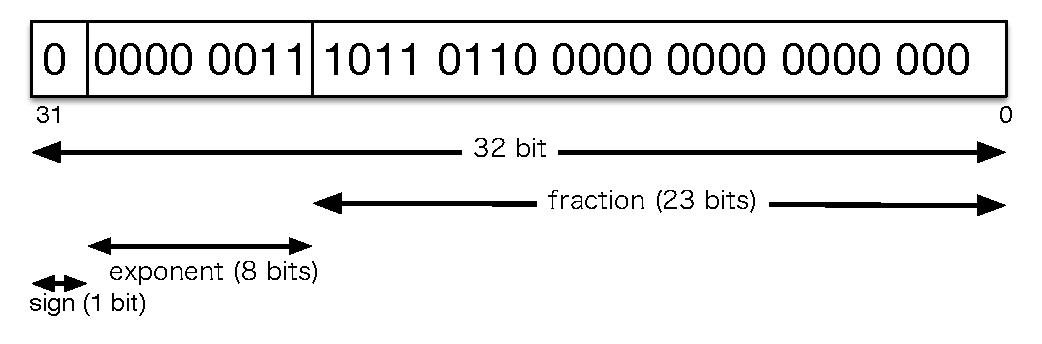
\includegraphics[scale=.4]{./Figure/elementaryCS-figFloatingPointFormat.eps}
  \end{center}
\end{frame}
\begin{frame}
\frametitle{Quiz: 浮動小数}
  \begin{itemize}
\item 実数の浮動小数表現をやってみてください
  \end{itemize}
  \begin{block}{宿題}
    \begin{itemize}
\item 35.75 を浮動小数で表現してみてください
    \end{itemize}
  \end{block}
\end{frame}
\begin{frame}
\frametitle{Quiz: 回答}
  \begin{itemize}
\item 2 進へ変換: 100011.11
\item 正規化: 1.0001111$\times 2^5$
\item 32 bit 形式に: {\scriptsize 0 0000 0101 0001 1110 0000 0000 0000 000}
    \begin{itemize}
\item 1. は省略
    \end{itemize}
\item 規格\href{http://ieeexplore.ieee.org/xpl/mostRecentIssue.jsp?punumber=2355}{\beamerbutton{IEEE 754}}では下駄 (bais) をはかせるので\(5+127=132\Rightarrow\) 1000 0100
\item 32 bit 形式に: {\scriptsize 0 1000 0100 0001 1110 0000 0000 0000 000}
  \end{itemize}
\end{frame}
\subsection{浮動小数の算術演算}
\begin{frame}[shrink,fragile]
\frametitle{浮動小数演算の変な現象}
  \begin{itemize}
\item machine\_epsilon.py を実行してみます
\item 結果が予測と少し違うことになります
\item この原因についてみていきます
  \end{itemize}
  \begin{lstlisting}[caption={machine\_epsilon.py}]
# Machine epsilon
import sys

epsilon, old, prod =1.0, 0.0, 0.0
cnt=0
while (prod!=1.0):
  print(epsilon)
  old = epsilon
  cnt=cnt+1
  epsilon=epsilon/2.0
  prod=epsilon+1.0
print("Calculated machine epsilon:",old)
print("System information in Python:",sys.float_info.epsilon)
  \end{lstlisting}
\end{frame}
\begin{frame}[shrink]
\frametitle{浮動小数数の算術演算}
  \begin{itemize}
\item 正規化した 2 つの浮動小数 \(X, Y\) を \(X=F_x\times 10^{e_x}, Y=F_y\times 10^{e_y}\) とする
\item 乗算: \(XY=(F_x\times 10^{e_x})(F_y\times 10^{e_y})=F_xF_y\times 10^{e_x+e_y}\)
\item 除算: \(\frac{X}{Y}=\frac{(F_x\times 10^{e_x})}{(F_y\times 10^{e_y})}=\frac{F_x}{F_y}\times 10^{e_x-e_y}\)
\item 加算\(\cdot\)減算: \(X\pm Y=(F_x\times 10^{e_x})\pm(F_y\times 10^{e_y})=(F_x\pm F_y\cdot 10^{e_y-e_x})\times 10^{e_x}\)
    \begin{itemize}
\item ただし,\(e_x\geq e_y\)
\item \(F_y\cdot 10^{e_y-e_x}\) は指数を大きい方に揃えたときの $Y$ の仮数
    \end{itemize}
\item 演算結果も正規化するので指数は調整が必要
  \end{itemize}
  \begin{example}[算術演算の例]
    \begin{columns}[t]
      \begin{column}{4.5cm}
        \begin{math}
          \begin{array}{cll}
&0.2184&\times 10^2\\
\times&0.2512&\times 10^2\\
\hline
&0.07998208&\times 10^4\\
=&0.7998208&\times 10^3\\
          \end{array}
        \end{math}
      \end{column}
      \begin{column}{4.5cm}
        \begin{math}
          \begin{array}{cll}
&0.2844&\times 10^3\\
+&0.4162&\times 10^1\\
\hline
&0.288562&\times 10^3\\
          \end{array}
        \end{math}
      \end{column}
    \end{columns}
  \end{example}
\end{frame}
%\begin{frame}
%\frametitle{算術演算の誤差}
%  \begin{itemize}
%\item 4 桁までしか記憶できないと仮定
%\item \(0.2844\cdot 10^3+0.4162\cdot 10^1=0.288562\cdot 10^3=(0.2885+0.000062)\cdot 10^3=0.2885\cdot 10^3+0.6200\cdot 10^{-1}\)
%\item \(0.288562\)が真の値となるが \(0.2885\) までしか記憶できないので
%\item \(0.6200\cdot 10^{-1}(=0.000062\cdot 10^3)\) について調整する必要がある
%  \end{itemize}
%  \begin{example}[\(0.2844\cdot 10^3+0.4162\cdot 10^1\)]
%    \begin{columns}[t]
%      \begin{column}{4.5cm}
%        \begin{math}
%          \begin{array}{cll}
%&0.2844&\times 10^3\\
%+&0.4162&\times 10^1\\
%\hline
%&0.288562&\times 10^3\\
%          \end{array}
%        \end{math}
%      \end{column}
%      \begin{column}{4.5cm}
%        \begin{math}
%          \begin{array}{cll}
%&0.2844&\times 10^3\\
%+&0.004162&\times 10^3\\
%\hline
%&0.288562&\times 10^3\\
%          \end{array}
%        \end{math}
%      \end{column}
%    \end{columns}
%  \end{example}
%\end{frame}
\section{誤差のおはなし}
\subsection{丸め誤差 (roundoff error)}
\begin{frame}[shrink]
\frametitle{誤差とは}
  \begin{itemize}
\item コンピュータの中では実数は有限個の 0 と 1 の組み合わせ(浮動小数)で表しています
\item なので,本来あるべき真値を適当な浮動小数で近似している
\item 近似値-真値 を誤差という
  \end{itemize}
\end{frame}
\begin{frame}[shrink]
\frametitle{丸め誤差 (roundoff error)}
  \begin{itemize}
\item 表現可能な範囲に丸めることを丸め誤差という
\item 演算結果も丸める
\item $Z$ を \(X\oplus Y\) の演算結果とする
\item $d$ 桁だけ記憶できるとして,先頭の $d$ 桁を $F$,残りを $f$ とすると,\(Z=F\cdot 10^{e_z}+f\cdot 10^{e_z-d}\)
\item $f$ の値で四捨五入することにして
    \begin{displaymath}
      \begin{array}{ll}
|f|<0.5 \mbox{のとき} & |Z|=|F|\cdot 10^{e_z-d}\\
|f|\geq 0.5 \mbox{のとき} & |Z|=|F|\cdot 10^{e_z-d}+\cdot 10^{e_z-d}
      \end{array}
    \end{displaymath}
\item 丸め誤差 $\epsilon_z$ とすれば
    \begin{displaymath}
      \begin{array}{ll}
|f|<0.5 \mbox{のとき} & |\epsilon_z|=|f|\cdot 10^{e_z-d}\\
|f|\geq 0.5 \mbox{のとき} & |\epsilon_z|=|1-f|\cdot 10^{e_z-d}
      \end{array}
    \end{displaymath}
  \end{itemize}
  \begin{example}[\(0.2844\cdot 10^3+0.4162\cdot 10^1\)]
    \begin{itemize}
\item \(0.2844\cdot 10^3+0.4162\cdot 10^1=0.2885\cdot 10^3+0.6200\cdot 10^{-1}\)
\item \(|Z|=0.2885\cdot 10^3+10^{3-4}=0.2886\cdot 10^3\)
\item \(|\epsilon_z|=|1-0.6200|\cdot 10^{3-4}=0.48\cdot 10^{-1}\)
    \end{itemize}
  \end{example}
\end{frame}
%\begin{frame}
%\frametitle{相対誤差 (relative error)}
%  \begin{itemize}
%\item 計算のコストだけでなくときには計算精度も重要になる
%\item 真の値 $x^t$,観測した値 $x$ として誤差 \(\epsilon_x=x^t-x\)
%\item \(|\epsilon_x|=|x^t-x|\) を絶対誤差という
%\item 相対誤差 \(r_x=\frac{\epsilon_{x}}{x}=\frac{x^t-x}{x}\) で精度を測る
%  \end{itemize}
%  \begin{example}[相対誤差の例]
%    \begin{itemize}
%\item \(x_t=9, x=10\) と \(y_t=999, y=1000\) の場合を考える
%\item $x$ と $y$ の誤差はどちらも \(-1\)
%\item $x$ と $y$ の相対誤差はそれぞれ \(r_x=\frac{-1}{10}, r_y=\frac{-1}{1000}\)
%    \end{itemize}
%  \end{example}
%\end{frame}
%\subsection{誤差の伝搬 (propagation of errors)}
%\begin{frame}
%\frametitle{誤差の伝搬 (propagation of errors)}
%  \begin{itemize}
%\item 誤差は計算中伝播して計算結果を不正確にしてしまう
%\item 算術式中の誤差がどう蓄積されていくかをみる
%\item ある数 $x, y$ としてそれぞれが誤差 \(\epsilon_x, \epsilon_y\) を持つとする
%\item このときの演算 \(x\oplus y\) の誤差 \(\epsilon_{x\oplus y}\) は
%    \begin{displaymath}
%\epsilon_{x\oplus y}=(x^t\oplus y^t)-(x\oplus y)
%    \end{displaymath}
%\item \(x^t\oplus y^t\) は真の演算結果で, \(x\oplus y\) は実際の結果
%\item 先の誤差の定義からこれが導ける
%  \end{itemize}
%\end{frame}
%\begin{frame}[shrink]
%\frametitle{誤差公式}
%  \begin{itemize}
%\item 各演算についてつぎの関係が成り立つ
%  \end{itemize}
%  \begin{theorem}[誤差公式]
%    \begin{math}
%      \begin{array}{lclclclcl}
%\scriptsize
%\epsilon_{x+y}&=&(x^t+y^t)-(x+y)&=&(x^t-x)+(y^t-y)&=&\epsilon_x+\epsilon_y\\
%\epsilon_{x-y}&=&(x^t-y^t)-(x-y)&=&(x^t-x)-(y^t-y)&=&\epsilon_x-\epsilon_y\\
%      \end{array}
%    \end{math}
%    \begin{math}
%      \begin{array}{lclclclcl}
%\epsilon_{xy}&=&(x^ty^t)-(xy)&=&(x+\epsilon_x)(y+\epsilon_y)-(xy)&=&\epsilon_x y+\epsilon_y x\\
%      \end{array}
%    \end{math}
%    \begin{math}
%      \begin{array}{lclclclcl}
%\epsilon_{\frac{x}{y}}&=&\frac{x^t}{y^t}-\frac{x}{y}&=&\frac{x^ty-y^tx}{y^ty}&=&\frac{(x+\epsilon_x)y-(y+\epsilon_y)x}{(y+\epsilon_y)y}\\
%&=&\frac{xy+\epsilon_xy-xy+x\epsilon_y}{y^2(1+\frac{\epsilon_y}{y})}&=&\frac{\epsilon_xy-\epsilon_yx}{y^2}\\
%      \end{array}
%    \end{math}
%    \begin{itemize}
%\item \(\epsilon_x\epsilon_y\) は十分小さいとして無視
%\item \(|\frac{\epsilon_y}{y}|\) は \(|\frac{\epsilon_y}{y}|\ll 1\) のとき無視
%\item これに各演算の丸め誤差 \(\alpha\) を加えたて誤差公式とする
%      \begin{itemize}
%\item たとえば 4 桁までしか記憶できないのであれば演算結果も 4 桁に丸められる
%      \end{itemize}
%    \end{itemize}
%  \end{theorem}
%\end{frame}
%\begin{frame}[shrink]
%\frametitle{相対誤差公式}
%  \begin{itemize}
%\item 相対誤差公式を導く
%\item 先の相対誤差の定義より
%    \begin{displaymath}
%r_{x\oplus y}=\frac{\epsilon_{x\oplus y}}{x\oplus y}
%    \end{displaymath}
%\item とすれば誤差公式よりつぎの相対誤差公式をえる
%  \end{itemize}
%  \begin{theorem}[相対誤差公式]
%    \begin{math}
%      \begin{array}{rclcl}
%r_{x+y}&=&\frac{\epsilon_x+\epsilon_y}{x+y}+\alpha&=&r_x\frac{x}{x+y}+r_y\frac{y}{x+y}+\alpha\\
%r_{x-y}&=&\frac{\epsilon_x-\epsilon_y}{x-y}+\alpha&=&r_x\frac{x}{x-y}+r_y\frac{-y}{x-y}+\alpha\\
%r_{xy}&=&\frac{\epsilon_x y+\epsilon_y x}{xy}+\alpha&=&r_x\ 1+r_y\ 1+\alpha\\
%r_{xy}&=&\frac{\frac{\epsilon_x y-\epsilon_y x}{y^2}}{\frac{x}{y}}+\alpha&=&r_x\ 1+r_y\ (-1)+\alpha
%      \end{array}
%    \end{math}
%  \end{theorem}
%\end{frame}
%\begin{frame}[shrink]
%\frametitle{誤差伝播の解析}
%  \begin{itemize}
%\item 相対誤差公式を使って誤差伝播の解析を行う
%  \end{itemize}
%  \begin{example}[和における誤差伝播]
%    \begin{itemize}
%\item \(r_0, r_1, r_2, r_3\) を実数 \(a_0,a_1,a_2,a_3\) の相対誤差とする
%\item \(S=(((a_0+a_1)+a_2)+a_3)\) の相対誤差を求める
%    \end{itemize}
%  \end{example}
%\end{frame}
\subsection{打ち切り誤差 (truncation error)}
\begin{frame}[shrink]
\frametitle{打ち切り誤差 (truncation error)}
  \begin{itemize}
\item コンピュータでは無限に繰り返して値をもとめることはできない
\item 有限回の計算で値を計算し,それを求める値の近似値としてもちいる
\item このときの誤差を打切り誤差という
  \end{itemize}
  \begin{example}[\(\sin(x)\)のマクローリン展開]
    \begin{itemize}
\item \(sin(x)=x-\frac{x^3}{3!}+\frac{x^5}{5!}-\frac{x^7}{7!}+\cdots+(-1)^{n}\frac{x^{2n+1}}{(2n+1)!}+\cdots\)
\item gnuplot で試してみてください
    \end{itemize}
  \end{example}
  \begin{example}[平方の計算]
    \begin{itemize}
%\item \href{run:newton.command}{\beamerbutton{ニュートン法}}
\item newton.py を参照
\item \(\sqrt{a}\) を求めてみる
\item \(f(x)=x^2-a\) として \(f(x)=0\) となる $x$ を求める
\item \(k+1\) 番目の近似値 \(x_{k+1}\) を
      \begin{displaymath}
x_{k+1} = x_k-\frac{f(x_k)}{f'(x_k)} = \frac{1}{2}(x_k+\frac{a}{x_k})
      \end{displaymath}
    \end{itemize}
  \end{example}
\end{frame}
%\section{まとめ}
%\begin{frame}[shrink,fragile]
%\frametitle{数値計算}
%  \begin{itemize}
%\item ここで取り上げたおはなしは数値計算(計算機科学の一分野)のなかの計算誤差をとりあげたもの
%\item シミュレーションなどではある関数の実際の数値を必要とする場合がある
%    \begin{itemize}
%\item 例えば,方程式 \(f(x)=0\) の $x$ を数値的に求める
%    \end{itemize}
%\item 数値計算の手順
%    \begin{itemize}
%\item 最初に適当な 1 次近似 \(x_0\) を選んで,
%\item より良い近似を求め,
%\item 適当な収束条件を満たすまで繰り返す (マシンイプシロンは収束条件の重要な指標)
%    \end{itemize}
%\item \(f\) は複雑なので数値的な解を求めるいろいろな算法を考察
%  \end{itemize}
%\end{frame}
